\graphicspath{{../05QuantumPhysics/pics/}}

\chapter{Quantum Physics}\label{ch:QuantumPhysics}
\lettrine[lines=2]{\color{darkocre}T}{he} first type of operators -- and
corresponding tensors -- that we encountered has a simple type:
\[
\op{L}\,\vec{a} = \vec{b}\,.
\]
It is a linear unary function mapping vectors into vectors.

As the next step, we will expand our toolset and study operators that take
two vectors as their input arguments. Their action on the arguments
can be symbolically written as follows:
\[
\op{L}\,\vec{a}\,\vec{b} = x
\]
if the results is a number, or
\[
\op{L}\,\vec{a}\,\vec{b} = \vec{c}
\]
if the results is another vector. We will start with the former case.


\section{Dol-Operator and Scalar Product}\label{sec:Dol}

Given a pair of vectors, for example arrows in a plane, we can
\emph{quantify their mutual orientation}. In other words, given two
vectors $\vec{a}$ and
$\vec{b}$, we can calculate a number that measures, for instance,
their \emph{degree of overlap}\index{Vectors!overlap} (or
\emph{alignment}) which tells how
much in common the vectors have with regard to their directions and
lengths.

We are looking for a binary operator $\op{\sigma}$ that yields a number
based on two vectors:
\[
\op{\sigma}\,\vec{a}\,\vec{b}=x\,.
\]
We will call this operator $\op{\sigma}$ \emph{dol}-operator\footnote{This is not a
standard terminology. }, based on the key letters of the phrase
``\underline{d}egree of \underline{o}ver\underline{l}ap''.

There are many methods to quantify mutual orientation of a pair
of vectors. One simple way is to measure the angle between them:
\[
\angle\,\vec{a}\,\vec{b} = \theta\,.
\]
However, we will limit our search for candidates to linear operators
or -- in the case of binary operator $\op{\sigma}$ -- to \emph{bilinear
operators}\index{Operator!bilinear}.
%\begin{tcolorbox}[colback=white!85!ocre, title=Problem]
\begin{exercise}\label{exe:angleOperatorNonlinear}
  Prove that the operator $\angle$ is not linear.
\end{exercise}
%\end{tcolorbox}

If the dol operator $\op{\sigma}$ is linear in each of its arguments, we must
have
\[
\op{\sigma}\,(2\vec{a})\,\vec{b} = \op{\sigma}\,(\vec{a}+\vec{a})\,\vec{b} =
\op{\sigma}\,\vec{a}\,\vec{b} + \op{\sigma}\,\vec{a}\,\vec{b} = 2
(\op{\sigma}\,\vec{a}\,\vec{b})\,.
\]
In general, we require
\[
\op{\sigma}\,(\alpha\vec{a})\,\vec{b} = \alpha (\op{\sigma}\,\vec{a}\,\vec{b})\,.
\]

In addition, we will not be concerned with the order in which the
vectors $\vec{a}$ and $\vec{b}$ are considered. Put differently, we
consider $\vec{a}$ aligned to $\vec{b}$ to the same degree as
$\vec{b}$ is aligned to $\vec{a}$. Mathematically this requirement is
written as follows:
\[
\op{\sigma}\,\vec{a}\,\vec{b} = \op{\sigma}\,\vec{b}\,\vec{a}\,.
\]
Functions and operators with this property are called
\emph{symmetric}\index{Function!symmetric}
in their arguments.

%\begin{tcolorbox}[colback=white!85!ocre, title=Note]
\begin{mybio}{Note}
Since angles are measured as clockwise (negative) or
counter-clockwise (positive), the
operator $\angle$ is not symmetric. It is called
\emph{anti-symmetric}:
\[
\angle\, \vec{a} \, \vec{b} = -(\angle\, \vec{b} \, \vec{a})\,.
\]
\end{mybio}
%\end{tcolorbox}

Finally, we recognize that some pairs of vectors are not overlapping. It
can be said that their degree of overlap is zero. Mutually
orthogonal vectors are example of vectors with zero overlap, they kind
of ``have nothing in common.'' Thus, we expect
\[
\op{\sigma}\,\vec{a}\,\vec{b} = 0
\]
if $\vec{a}\perp\vec{b}$.

Now every vector can be written in the form
\[
\vec{a} = a\vec{u}_a\,,
\]
where $a$ is the length of the vector, $\vec{u}_a$ is the unit-length
vector pointing in the same direction as $\vec{a}$. Similarly for
$\vec{b}$:
\[
\vec{b} = b\vec{u}_b\,.
\]
Since dol-operator $\op{\sigma}$ is linear in each argument, we can write
\[
\op{\sigma}\,\vec{a}\,\vec{b} = ab (\op{\sigma}\,\vec{u}_a\,\vec{u}_b)\,.
\]

The problem is thus reduced to quantifying mutual overlap of unit
vectors $\vec{u}_a$ and $\vec{u}_b$. Although we can't use the angle
between these vectors directly, we can use some function of the angle:
\[
\op{\sigma}\,\vec{u}_a\,\vec{u}_b = f\,\theta\,.
\]
Firstly, this function has to be periodic since changing the mutual angle by
$2\pi$ results in the same mutual orientation. Secondly, for
orthogonal vectors the function must return zero degree of overlap:
\[
f\, (\pi/2) = 0\,.
\]

After some search and reflection, a reasonable candidate function
can be written in the following way:
\[
f\, \theta =\cos\theta\,.
\]
We arrived at the traditional operation of \emph{scalar
product}\index{Vectors!scalar product}
(numeric product) of two vectors. For scalar product a special
\emph{infix notation}\index{Notation!infix} is conventionally used:
\[
\colorboxed{red}{
  \op{\sigma}\,\vec{a}\,\vec{b} = \vec{a}\cdot\vec{b}=ab\cos\theta\,.
  }
\]

What is the geometric meaning of scalar product? As shown in the
Figure \ref{fig:scalarProductMeaning}, one way to interpret the scalar
product $\vec{a}\cdot\vec{b}=ab\cos\theta$ is to consider it as the
 area of a rectangle with sides $a$ and $b\cos\theta$. A special care
 must be taken for cases when the mutual angle is greater than $\pi$.


\begin{figure}[htbp]
  \centering
  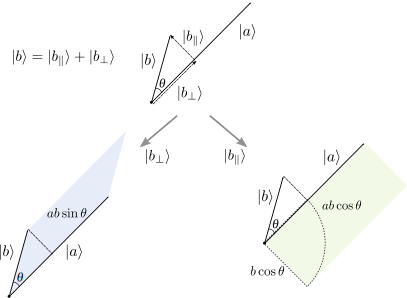
\includegraphics[scale=1.0]{scalarProductMeaning}
  \caption{Scalar product of two vectors can be given a simple
    geometric interpretation as the unsigned area of a rectangle with the
    sides $a$ and $b\cos\theta$ or with the sides $a\cos\theta$ and $b$.}
  \label{fig:scalarProductMeaning}
\end{figure}

\section{Scalar Product Properties}\label{sec:ScalarProductProperties}
The expression for scalar product of two vectors
\[
\vec{a}\cdot\vec{b} = ab\cos\theta
\]
implies the \emph{commutativity}\index{Commutativity} of scalar product operation:
\[
\vec{b}\cdot\vec{a} = ba\cos\theta = ab\cos\theta = \vec{a}\cdot\vec{b}.
\]

%\begin{tcolorbox}[colback=white!90!ocre, title=Non-commutativity]
\begin{mybio}{Non-commutativity}
Commutativity is a familiar property, present for both addition and
multiplication of numbers. It is sometimes accepted as a natural
property of any multiplication-like operation. This view is limiting,
however, and we will later learn how to multiply objects without
commutativity:
\[
A\bowtie B \ne B\bowtie A\,.
\]
Here we used an arbitrary infix symbol $\bowtie$ to denote non-commutative
product of some objects $A$ and $B$. What exactly those objects are
and what their product might mean will be clear when we introduce them
properly. Right now we want to highlight the non-commutativity as a
valid property of many binary operations.
\end{mybio}
%\end{tcolorbox}

Besides commutativity scalar product has other useful
properties. First, it is trivial to demonstrate that we can ``pull out''
constant scale factors of vectors:
\[
(\alpha\vec{a})\cdot\vec{b}=\alpha(\vec{a}\cdot\vec{b})\,
\]
and similarly
\[
\vec{a}\cdot(\beta \vec{b})=\beta(\vec{a}\cdot\vec{b})\,.
\]

To arrive at the second important property of scalar product, recall
that in the geometric
interpretation of the scalar product we had expressions
\[
b\cos\theta = b_\parallel\quad\textrm{ or }\quad a\cos\theta = a_\parallel\,,
\]
where $b_\parallel$ is the part of the vector $\vec{b}$ parallel to
$\vec{a}$ ($a_\parallel$ is the part of the vector $\vec{a}$ parallel to
$\vec{b}$.)

Now, if the vector $\vec{a}$ is ``made from'' two other vectors
\[
\vec{a}=\vec{c}+\vec{d}\,,
\]
then, as illustrated in the Figure (\ref{fig:scalarProductProperty}),
\[
a_{\parallel}=c_{\parallel}+d_{\parallel}\,,
\]
where all terms represent parts of the respective vectors parallel to
the vector $\vec{b}$. Of course, the angles between the vectors
$\vec{a}$, $\vec{c}$, $\vec{d}$ and the vector $\vec{b}$ may all be different:
\[
a_{\parallel}=a\cos\theta = c\cos\phi + d\cos\psi\,.
\]
Given that
\[
\vec{a}\cdot\vec{b} = ab\cos\theta\,,\quad
\vec{c}\cdot\vec{b} = cb\cos\phi\,,\quad
\vec{d}\cdot\vec{b} = db\cos\psi\,,
\]
we arrive at the \emph{distributive property}\index{Distributivity}
of scalar product:
\[
(\vec{c}+\vec{d})\cdot\vec{b}=\vec{a}\cdot\vec{b}=(\vec{c}\cdot\vec{b})+(\vec{d}\cdot\vec{b})\,.
\]
\begin{figure}[htbp]
  \centering
  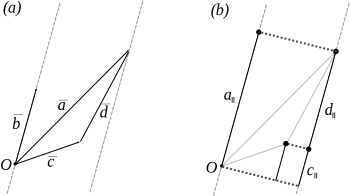
\includegraphics[scale=1.0]{scalarProductProperty}
  \caption{Simple geometric construction illustrates the distributive
    property of scalar product:
    $(\vec{c}+\vec{d})\cdot\vec{b}=(\vec{c}\cdot\vec{b})+(\vec{d}\cdot\vec{b})$.}
  \label{fig:scalarProductProperty}
\end{figure}

Putting it all together, we can express the properties of scalar
product in a single expression:
\[
(\alpha\vec{a}+\beta\vec{b})\cdot\vec{c}=\vec{c}\cdot(\alpha\vec{a}+\beta\vec{b})=\alpha(\vec{a}\cdot\vec{c})+\beta(\vec{b}\cdot\vec{c})\,.
\]

%\begin{tcolorbox}[colback=white!90!ocre, title=Orthogonality]
\begin{mybio}{Orthogonality}
We might wonder whether we can define, instead of degree of alignment,
some measure of orthogonality for a pair of vectors? Indeed, a
reasonable candidate might be (using infix notation):
\[
\vec{a\,}\vdash\,\vec{b}=ab\sin\theta\,.
\]
While this is an acceptable definition, the expression on the right-hand
side appears in a different, more powerful and useful, operation of
\emph{outer product} of two vectors. The concept of outer product is
related to the concept of \emph{tensor product}\index{Tensor!product}
(see Section \ref{sec:TensorProduct}) but is beyond the scope of this
book.
\end{mybio}
%\end{tcolorbox}

Using the properties of scalar product and expanding vectors in terms
of the basis vectors, we can write scalar product in terms of vector
components. First write

\[
(a_{1}\vec{e}_{1}+a_{2}\vec{e}_{2})\cdot\vec{b}=a_{1}(\vec{b}\cdot\vec{e}_{1})+a_{2}(\vec{b}\cdot\vec{e}_{2})\,.
\]
Next, expand $\vec{b}$ to find
\[
(b_{1}\vec{e}_{1}+b_{2}\vec{e}_{2})\cdot\vec{e}_{i}=b_{1}(\vec{e}_{1}\cdot\vec{e}_{i})+b_{2}(\vec{e}_{2}\cdot\vec{e}_{i})\,.
\]
Finally, combining the results of two previous steps, we arrive at
the expression
\[
\vec{a}\cdot\vec{b}=a_{1}b_{1}(\vec{e}_{1}\cdot\vec{e}_{1})+a_{1}b_{2}(\vec{e}_{2}\cdot\vec{e}_{1})+a_{2}b_{1}(\vec{e}_{1}\cdot\vec{e}_{2})+a_{2}b_{2}(\vec{e}_{2}\cdot\vec{e}_{2})\,.
\]
For arbitrary basis vectors the scalar product is then given by
\[
\colorboxed{red}{
  \vec{a}\cdot\vec{b}=a_{1}b_{1}e_{1}^{2}+(a_{1}b_{2}+a_{2}b_{1})e_{1}e_{2}\cos\theta+a_{2}b_{2}e_{2}^{2}\,,
  }
\]
where $\theta$ is the angle between the basis vectors $\vec{e}_{1}$
and $\vec{e}_{2}$. For a special case of orthonormal basis the
scalar product takes the simplest form:
\[
\colorboxed{red}{
  \vec{a}\cdot\vec{b}=a_{1}b_{1}+a_{2}b_{2}=a_ib_i\,.
  }
\]
But in general we must know the values for all products $\vec{e}_{i}\cdot\vec{e}_{j}$.
A special notation is used for these products:
\[
\eta_{ij}=\vec{e}_{i}\cdot\vec{e}_{j}=\op{\sigma}\,\vec{e}_i\,\vec{e}_j\,.
\]
This notation allows a more compact way of writing scalar
product\index{Vectors!scalar product} for general
basis:
\[
\colorboxed{red}{
  \vec{a}\cdot\vec{b}=\eta_{ij}a_{i}b_{j}\,.
}
\]

%\begin{tcolorbox}[colback=white!90!ocre, title=Scalar Product
%Components]
\begin{mybio}{Scalar Product Components}
Let's take a look how the derivation of the last result can be done
using index notation.
\[
\vec{a}\cdot\vec{b} = (a_i\vec{e}_i)\cdot\vec{b} = a_i(\vec{e}_i\cdot\vec{b})\,.
\]
Expanding $\vec{b}$, we get
\[
\vec{a}\cdot\vec{b} = a_i(\vec{e}_i\cdot\lbrack b_j\vec{e}_j\rbrack) = a_i(b_j\lbrack\vec{e}_i\cdot\vec{e}_j\rbrack)\,.
\]
We thus showed that
\[
\vec{a}\cdot\vec{b} = a_ib_j\vec{e}_i\cdot\vec{e}_j\,.
\]
% \cdot (b_j\vec{e}_j)=a_ib_j(\vec{e}_i\cdot\vec{e}_j)\,.

In the process we had to use twice the distributive property of the
scalar product, as well as distributive property of number
multiplication.
\end{mybio}
%\end{tcolorbox}

%\begin{tcolorbox}[colback=white!90!ocre, title=Problem]
\begin{exercise}\label{exe:projectorOperatorFromScalarProduct}
  In the index form of scalar product of two vectors
  \[
  \vec{a}\cdot\vec{b} = (a_ib_j)(\vec{e}_i\cdot\vec{e}_j)
  \]
  we observe the expression with two indices:
  \[
  \beta_{ij} = a_ib_j\,.
  \]
  Can $\beta_{ij}$ represent the components of some linear
  operator $\op{\beta}$? If so, how does this operators act on vectors?
\end{exercise}
%\end{tcolorbox}


\section{Inner Operations}
The following fact is easy to take for granted and overlook:
\emph{Vectors are not used by themselves. They need numbers.}  Without
multiplying a vector by a number, we could not write the
simplest expansion of a vector $\vec{a}$ in a basis:
\begin{equation*}
	\vec{a} = a_1\vec{e}_1 + a_2\vec{e}_2\,.
\end{equation*}

Note that all operations we considered so far never took us
outside of the combined realm of numbers $\mathbb{R}$ and vectors
$\vsp{A}$. Indeed, a product of a number and a vector $\alpha\vec{a}$
uses one element of each space, and produces a vector. Similarly, a
sum of two vectors $\vec{a} + \vec{b}$ takes two elements from
$\vsp{A}$ and returns another element of
$\vsp{A}$. Finally, the dol-operator $\op{\sigma}$ takes two  elements from
$\vsp{A}$ and returns an element of  $\mathbb{R}$. These points are
illustrated in the Figure \ref{fig:arrowsSpaceAndNumbers}(a).

Another way to look at this is to notice that in the hierarchy of
mathematical objects the operations we considered so far never took us
up the ladder of \emph{ranks}\index{Tensor!rank}, as illustrated in the Figure
\ref{fig:arrowsSpaceAndNumbers}(b). At the lowest level we have
\emph{rank-0} elements -- numbers. The first ladder corresponds to the
\emph{rank-1} elements -- vectors. One step higher we have
\emph{rank-2} elements -- tensors of the second rank, and so on.

All operations that \emph{do not} result in the element of higher rank
are called \emph{inner operation}. For instance, scalar product of vectors is
often called \emph{inner product}\index{Product!inner}\footnote{There also exists an
\emph{outer product}, which is related to \emph{tensor product}\index{Product!tensor}
discussed in Section \ref{sec:TensorProduct}.}. The
phrase \emph{inner sum} is not used for the binary operator $(+)$.

\section{Conjugate Objects}\label{sec:conjugateObjects}

Starting from the dol-operator
\[
\op{\sigma}\,\vec{a}\,\vec{b}=x
\]
we can arrive at an important notion of \emph{conjugate}\index{Conjugate} objects.
Conjugate objects, roughly speaking, are objects that are somehow
related via a simple rule. We will study this notion using vectors.

For every vector $\vec{a}$ there exists a mathematical object, related
to $\vec{a}$ via the dol-operator. To see this, we first need to
revisit the idea of \emph{partial application}\index{Partial
  application}, discussed in subsection
\ref{subsec:PartialApplication}. This time, however, we will extend
the idea of partial application to binary operators.

\subsection{Partial Application}\label{subsec:PartialApplication}

Given a pair of vectors, the dol-operator yields a number:
\[
\op{\sigma}\,\vec{a}\,\vec{b} = x\,.
\]

What happens when we provide only one vector, leaving the second input
slot of $\op{\sigma}$ empty (the box here indicates a missing second argument):
\[
\op{\sigma}\,\vec{a}\,\Box\,?
\]
This is called \emph{partial application} of the operator $\op{\sigma}$.
This construction has the behavior of a unary operator that maps any
vector into a number:
\[
\vec{c}\,\overset{\op{\sigma}\,\vec{a}}{\longrightarrow}y\,.
\]
%\begin{tcolorbox}[colback=white!90!ocre, title=Linear Operator]
\begin{mybio}{Linear Operator}
  The unary operator
  \[
  \op{L}_a = \op{\sigma}\,\vec{a}
  \]
  is a \emph{linear operator}\index{Operator!linear}:
  \[
  \op{L}_a (\vec{b} + \vec{c}) = (\op{L}_a\vec{b}) + (\op{L}_a\vec{c})\,.
  \]
\end{mybio}
%\end{tcolorbox}
We will use a special notation for the partially applied operator:
\[
\colorboxed{red}{
  \vecl{a}=\op{\sigma}\,\vec{a}\,.
}
\]
The action of a unary operator $\overset{\leftarrow}{a}$ on any
vector is then naturally defined as
\[
\vecl{a}\,\vec{b}=\op{\sigma}\,\vec{a}\,\vec{b}=ab\cos\theta\,.
\]
Notice that in the left-most expression the operator $\vecl{a}$ and
the argument vector $\vec{b}$ are separated by space, in agreement
with the notation for application of functions and operator to their
arguments.

\begin{figure}[htbp]
  \centering
  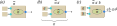
\includegraphics[scale=1.0]{doalPartialApplication}
  \caption{(a) The dol-operator is a binary operator linear in each of
    its arguments (\emph{bilinear}). (b) When only one argument is supplied, the
    operator becomes \emph{partially applied} and is denoted using the
    \emph{conjugate vector} notation $\vecl{a}$. (c) Applied to two vector
    arguments (\emph{fully applied}), dol-operator yields a number
    -- scalar product of the vectors.}
  \label{fig:doalPartialApplication}
\end{figure}
All three possible ``states'' of the dol-operator $\op{\sigma}$ are
illustrated in the Figure \ref{fig:doalPartialApplication}. The middle
state of partial application corresponds to a linear operator built
from the first input vector $\vec{a}$ and as denoted as
$\vecl{a}$. The operator $\vecl{a}$ is called the \emph{conjugate}\index{Conjugate}
to a vector $\vec{a}$. The conjugation is understood \emph{relative
to the binary operator} $\op{\sigma}$.
\begin{mybio}{Quantum Notation}
  In quantum physics vectors and their duals are used to describe
  properties of quantum systems. Paul Dirac introduced a very powerful
  notation for these vectors, called \emph{bra} and \emph{ket}
  vectors. Ket vectors correspond to contravariant arrow-vectors and
  are denoted as follows:
  \[
  \vec{a}\quad\longrightarrow\quad \ket{a}\,.
  \]
  Bra vectors correspond to covariant vectors and are denoted as
  \[
  \vecl{a}\quad\longrightarrow\quad \bra{a}\,.
  \]
  Scalar product of bra and ket vectors is then written using
  \emph{brackets}:
  \[
  \vecl{a}\,\vec{a} = \langle a | a \rangle\,.
  \]
\end{mybio}


\section{Conjugate Vectors}\label{sec:conjugateVectors}

The notation for the conjugate vectors\index{Conjugate!vector} is
suggestive for a reason.
The left-pointing arrow on top indicates that this is a vector. This
might be surprising, since we just convinced ourselves that $\vecl{a}$
is a linear operator. To
convince ourselves that $\vecl{a}$ is also a vector, we must check
whether the conjugate of vectors possess defining properties of
vectors. Let's do it.

To demonstrate that we can add two conjugate vectors -- which are also
linear operators -- we must describe
how to add operators. Operators are essentially functions, and we
already understand how to add functions of a numerical arguments (go
back to subsection \ref{subsec:FunctionComposition} if you need a
refresher.)

We can add two operators\index{Operator!addition}, $\vecl{a}$ and $\vecl{b}$,
in a similar way:
\[
\vecl{a}+\vecl{b} = \vecl{c}\,,
\]
where
\[
\vecl{c}\vec{d}=(\vecl{a}+\vecl{b})\vec{d}=(\vecl{a}\vec{d})+(\vecl{b}\vec{d})\,.
\]
As a sidenote, we point out once more that the addition operation
``$+$'' in $\vecl{a}+\vecl{b}$ is applied
to a new type of mathematical objects -- conjugate vectors. The addition
operator in $\vecl{a}\vec{d}+\vecl{b}\vec{d}$ is applied to usual
numbers.

It is easy to see how conjugate vectors can be multiplied by numbers:
\[
\alpha\vecl{a} = \vecl{b}\,,
\]
where
\[
\vecl{b}\vec{c}=\alpha(\vecl{a}\vec{c})\,.
\]

\subsubsection*{Conjugate Basis}
If conjugate objects are vectors, they must have some basis.
The basis for conjugate vectors\index{Basis!conjugate} can be taken by
conjugating any basis from the arrow-vectors:
\[
\colorboxed{red}{
  \vecl{e}_{1}=\op{\sigma}\,\vec{e}_{1}\,,\quad\vecl{e}_{2}=\op{\sigma}\,\vec{e}_{2}\,.
  }
\]
The linearity of the operator $\op{\sigma}$ for both arguments results
in the following relation
\[
\vecl{a}=\op{\sigma}\,\vec{a}=\op{\sigma}\,(a_{1}\vec{e}_{1}+a_{2}\vec{e}_{2})=a_{1}\vecl{e}_{1}+a_{2}\vecl{e}_{2}\,.
\]
In other words, \emph{any conjugate vector can be expanded in terms of
some basis conjugate vectors} $\lbrace \vecl{e}_i\rbrace$.
%\begin{tcolorbox}[colback=white!90!ocre, title=Problem]
\begin{exercise}\label{exe:expansionInConjugateBasis}
  Derive the relationship
  \[
  \vecl{a} = a_1\vecl{e}_1 + a_2\vecl{e}_2
  \]
  in more details, without leaving out steps.
\end{exercise}
%\end{tcolorbox}


%% %\begin{tcolorbox}[colback=white!90!ocre, title=Problem]
%% \begin{exercise}
%%   Suppose we know that vectors $\vec{a}$ and $\vec{b}$ are
%%   \emph{independent} (not parallel):
%%   \[
%%   \vec{a}\,\nparallel\,\vec{b}\,.
%%   \]
%%   Show that their conjugates $\vecl{a}$ and $\vecl{b}$ are also
%%   independent.
%% \end{exercise}
%% %\end{tcolorbox}

\subsubsection*{Component Transformation}
Finally, we must show that the components of any conjugate vector
change properly when the (conjugate) basis is switched.

We start by writing the same operator $\vecl{a}$ in
different bases:
\[
\vecl{a}=a_{1}\vecl{e}_{1}+a_{2}\vecl{e}_{2}=a'_{1}\veclp{e}_{1}+a'_{2}\veclp{e}_{2}\,.
\]

Here
\[
\veclp{e}_{1}=\op{\sigma}\,\vecp{e}_{1}\,,\quad\veclp{e}_{2}=\op{\sigma}\,\vecp{e}_{2}\,.
\]
Expanding the primed basis in terms of the non-primed, and using the
linearity of the operator $\op{\sigma}$ for all arguments, we get
\[
\veclp{e}_{1}=\op{\sigma}\,\vecp{e}_{1}=E_{11}\vecl{e}_{1}+E_{12}\vecl{e}_{2}\,,
\]
\[
\veclp{e}_{2}=\op{\sigma}\,\vecp{e}_{2}=E{}_{21}\vecl{e}_{1}+E_{22}\vecl{e}_{2}\,.
\]
Plugging these equations into the expansion of $\text{\ensuremath{\overset{\leftarrow}{a}}}$,
after grouping the terms, we arrive at
\[
\vecl{a}=a_{1}\vecl{e}_{1}+a_{2}\vecl{e}_{2}=(a'_{1}E_{11}+a'_{2}E_{21})\vecl{e}_{1}+(a'_{1}E_{12}+a'_{2}E_{22})\vecl{e}_{2}\,.
\]
Comparing the coefficients in front of the basis vectors, we conclude
that
\[
a_{1}=a'_{i}E_{i1}\,,
\]
\[
a_{2}=a'_{i}E_{i2}\,.
\]
In a more compact form:
\[
\colorboxed{red}{
  a_{j}=a'_{i}E_{ij}\,.
}
\]
This is the same form we obtained before for arrow-vectors, with the
only (unessential) difference of notation -- using $E$ instead of
$L$ to denote the relation between the ``old'' and ``new'' bases.

The conclusion is as follows: \emph{The conjugate vectors have completely
analogous properties as the arrow-vectors, when referred to their own
conjugate bases}.

We thus showed that vectors in plane have ``conjugate image'' --
a set of linear operators which also behave like vectors. These
conjugate vectors belong to the special vector
space\index{Vector!space!dual} called \emph{conjugate vector space} or
\emph{dual vector space}. The ``usual'' vector space is denoted as
$\vsp{A}$ and its dual companion is denoted as $\vspd{A}$.
The relationship between the ``original''
and the \emph{conjugate/dual} space is illustrated in the
Figure \ref{fig:arrowsConjugateSpace}.

\begin{SCfigure}%[htbp]
  %\centering
  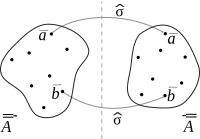
\includegraphics[scale=1.0]{arrowsConjugateSpace}
  \caption{Conjugate vectors like $\vecl{a}$ form a conjugate space
    which we denote $\vspd{A}$. It is \emph{conjugate} or \emph{dual}
    to the ``usual'' vectors space $\vsp{A}$.}
  \label{fig:arrowsConjugateSpace}
\end{SCfigure}


\section{Operators Are Also Vectors}\label{sec:operatorsAsVectors}

Starting with the binary bilinear dol-operator $\op{\sigma}$, we obtained unary
linear operators using partial application\index{Partial application}
\[
\vec{a}\quad\Longrightarrow\quad \vecl{a} = \op{\sigma}\,\vec{a}\,.
\]
We then showed that all
such linear operators $\vecl{a}$ behave
like vectors. They can be multiplied by a number, added, written in
terms of some basis, and have components that transform according to a
special rule:
\[
\vecl{a} = a_i\vecl{e}_i = a'_j\vecl{e}'_j\,
\]
where
\[
\colorboxed{red}{
  a_i = a'_jE_{ji}\,.
}
\]
We discovered a natural connection (\emph{duality}) between
every arrow-vector and its conjugate vector:
\[
\vec{a}\overset{\op{\sigma}}{\longleftrightarrow}\overset{\leftarrow}{a}\,.
\]

We can start with unary linear operators, without specifying
their origin, and show that they behave like vectors. We will do it
now.

\begin{SCfigure}%[htbp]
  %\centering
  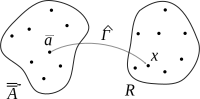
\includegraphics[scale=1.0]{linearOperatorsToNumbers}
  \caption{Some linear operators map vectors into numbers:
    $\op{\Gamma}\, \vec{a} = x$. Such operators form a vector space of
    their own.}
  \label{fig:linearOperatorsToNumbers}
\end{SCfigure}


Imagine \emph{all possible} unary linear
operators\index{Operator!unary} that map vectors into
numbers (see Figure \ref{fig:linearOperatorsToNumbers}). Let us denote
some such operator as $\op{\Gamma}$:
\[
\op{\Gamma}\,\vec{a}=x_a\,,
\]
\[
\op{\Gamma}\,(\alpha\vec{a})=\alpha(\op{\Gamma}\,\vec{a})=\alpha x_a\,.
\]
For $\vec{c}=\vec{a}+\vec{b}$:
\[
\op{\Gamma}\,\vec{c}=(\op{\Gamma}\,\vec{a})+(\op{\Gamma}\,\vec{b})=x_a+x_b=x_c\,.
\]
All $x_a$, $x_b$, and $x_c$ are real numbers.

We can demonstrate that operators like $\op{\Gamma}$ can be added:
\[
\op{\Gamma} = \op{\Gamma}_1 + \op{\Gamma}_2
\]
and they can be multiplied  by numbers:
\[
\op{\Gamma}_2 = \alpha\op{\Gamma}_1\,.
\]
We can also find basis and expand an arbitrary operator in that
basis:
\[
\op{\Gamma} = \gamma_1\op{\Gamma}_1 + \gamma_2\op{\Gamma}_1 + \ldots +
\gamma_n\op{\Gamma}_n = \gamma_i\op{\Gamma}_i
\]
 and establish the transformation rule for the
components $\gamma_i$ between different bases. In effect, we
will demonstrate that unary linear
operators of the same type as $\op{\Gamma}$ (mapping arrow-vectors
into numbers) behave like vectors and therefore must be considered as
such.

%\begin{tcolorbox}[colback=white!90!ocre, title=Reminder]
\begin{myrem}{Reminder}
When we say that an operator $\op{\Gamma}$ is given or known, we
mean that we know how it acts on \emph{any vector} $\vec{a}$:
\[
\op{\Gamma}\,\vec{a} = x_a\,.
\]
\end{myrem}
%\end{tcolorbox}

\subsubsection*{Addition}
If we know two operators $\op{\Gamma}_1$ and $\op{\Gamma}_2$, then
making sense of their \emph{operator sum}\index{Operator!addition}
$\op{\Gamma}=\op{\Gamma}_1 + \op{\Gamma}_2$ is easy:
\[
\op{\Gamma}\,\vec{a} =
(\op{\Gamma}_1\,\vec{a})+(\op{\Gamma}_2\,\vec{a})
= x_a + y_a\,,
\]
where $x_a = \op{\Gamma}_1\,\vec{a}$ and $y_a=\op{\Gamma}_2\,\vec{a}$.

\subsubsection*{Multiplication}
If we know the operator $\op{\Gamma}_1$ then
making sense of the product of that operator with any number
$\op{\Gamma}=\alpha\op{\Gamma}_1$ is easy:
\[
\op{\Gamma}\,\vec{a} = \alpha(\op{\Gamma}_1\,\vec{a}) = \alpha x_a\,,
\]
where $x_a = \op{\Gamma}_1\,\vec{a}$.

\subsubsection*{Finding Basis}
Using the linearity of the operators $\op{\Gamma}$, we can apply it to an
arbitrary vector $\vec{a}$ as follows:
\[
\op{\Gamma}\,\vec{a} = \op{\Gamma}\, (a_i\vec{e}_i) =
a_i\,(\op{\Gamma} \vec{e}_i)\,.
\]
The last expression states that to know the action of the operator
$\op{\Gamma}$ on an arbitrary vector $\vec{a}$ it is sufficient to
specify its action on all basis vectors $\vec{e}_i$. In other words,
the operator $\op{\Gamma}$ is fully specified if we know a set of
numbers
\[
\colorboxed{red}{
  \gamma_i = \op{\Gamma}\,\vec{e}_i\,.
}
\]
Notice how similar this last expression is to the definition of
components $L_{ij}$ of a linear operator $\op{L}$.
 %\begin{tcolorbox}[colback=white!90!ocre, title=Operators and
%Vectors]
\begin{mybio}{Operators and Vectors}
A vector $\vec{a}$ is completely determined if we specify its
components in a given basis:
\[
\vec{a} = a_i\vec{e}_i\,.
\]
A linear operator $\op{\Gamma}$ that maps vectors into numbers
\[
\vec{a}\quad\overset{\op{\Gamma}}{\longrightarrow}\quad x_a
\]
is completely determined if we specify its action on basis vectors:
\[
\gamma_i = \op{\Gamma}\,\vec{e}_i\,.
\]
This makes the similarity between vectors and operators $\op{\Gamma}$
stronger.
\end{mybio}
%\end{tcolorbox}

 Let's expand the input vector $\vec{a}$ in a different basis:
 \[
 \vec{a} = a'_j\vecp{e}_j\,.
 \]
 In this case the action of the linear operator $\op{\Gamma}$ will be
\[
\op{\Gamma}\, (a'_j\vecp{e}_j) = a'_j\,(\op{\Gamma} \vecp{e}_j) = a'_j\gamma'_j\,.
\]
Here $\gamma'_j = \op{\Gamma}\,\vecp{e}_j$.

The relation between the components $a_i$ and $a'_i$ of the
contravariant vector $\vec{a}$ is known; the
relation between the values $\gamma_i$ and $\gamma'_j$ is then
easily found:
\[
\gamma'_i = \op{\Gamma} \vecp{e}_i = \op{\Gamma} (E_{ij}\vec{e}_j) = E_{ij} \gamma_j\,,
\]
and, in a similar way:
\[
\gamma_i = \op{\Gamma} \vec{e}_i = \op{\Gamma} (E'_{ij}\vecp{e}_j) = E'_{ij} \gamma'_j\,.
\]
These relations correspond to the \emph{covariant vector}.

%\begin{tcolorbox}[colback=white!90!ocre, title=Covariant Vectors]
\begin{mybio}{Covariant Vectors}
The components of contravariant vectors allow us to ``assemble'' them
 from the ``building blocks'' -- basis vectors:
\[
\vec{a} = a_i\vec{e}_i\,.
\]
The basis vectors and all other vectors constructed from them all
\emph{live in the same vector space}, which we denoted $\vsp{A}$ --
the space of \emph{contravariant vectors}\index{Vector!contravariant}.

\vspace{0.2cm}
Unary linear operators, including all conjugate vectors, belong to a
different vector space -- \emph{conjugate} or \emph{dual}\index{Vector!space!dual} to
$\vsp{A}$. We denoted this vectors space as $\vspd{A}$. The Figure
\ref{fig:arrowsConjugateSpace} illustrates this point.

This implies that it is \emph{incorrect} to write
\[
\op{\Gamma} = \gamma_i \vec{e}_i\,.\quad\textrm{ (\emph{incorrect!}) }
\]
Conjugate space $\vspd{A}$ has its own basis (or bases).
\end{mybio}
%\end{tcolorbox}

It is important to understand that the coefficients $\gamma_i$ and
$\gamma'_j$ refer to bases used for contravariant vectors (bases
$\lbrace \vec{e}_i\rbrace$ and $\lbrace \vecp{e}_i\rbrace$). They
can also refer to bases used for covariant vectors. Let's find
some such basis related to the coefficients $\gamma_i$.

Every covariant vector $\op{\Gamma}$ is completely determined if we know its
action on \emph{all} basis contravariant vectors
$\vec{e}_i$. Therefore, to specify some basis vectors for $\op{\Gamma}$ we
should find certain covariant vectors that can be used as ``building
blocks'' for $\op{\Gamma}$. As a matter of fact, we already
encountered basis covariant vectors when we discussed dol-operator and
 conjugate
vectors of $\vec{e}_i$. We now will define similar vectors without
referring to dol operator $\op{\sigma}$. Specifically, the first basis
vector $\op{\Gamma}_1$ for covariant vectors acts on $\vec{e}_i$ as follows:
\begin{eqnarray}
  \op{\Gamma}_1\,\vec{e}_1 & = & 1\,\\
  \op{\Gamma}_1\,\vec{e}_2 & = & 0\,\\
  \op{\Gamma}_1\,\vec{e}_3 & = & 0\,\\
  \ldots
\end{eqnarray}
Thus, $\op{\Gamma}_1$ returns zero for all basis vectors except for
$\vec{e}_1$. Similarly, we define the second basis covariant vector
$\op{\Gamma}_2$ to return zero for all basis vectors except for
$\vec{e}_2$, and so on for other basis covariant vectors. A compact
way to express this idea uses index notation:
\[
\colorboxed{red}{
  \op{\Gamma}_i\,\vec{e}_j = \delta_{ij}\,.
}
\]
Here $\delta_{ij}$ is the Kronecker delta, introduced in Chapter
\ref{ch:NumbersFunctions} on page \pageref{subsec:multiindexObjects}.

Having defined this covariant basis, we can write now
\[
\op{\Gamma} = \gamma_1\op{\Gamma}_1 + \gamma_2\op{\Gamma}_1 + \ldots \gamma_n\op{\Gamma}_n=\gamma_j\op{\Gamma}_j\,.
\]
Clearly,
\[
\op{\Gamma}\,\vec{e}_i = \gamma_i\,.
\]
(To demonstrate this quickly, recall that
$\op{\Gamma}\,\vec{e}_i=\gamma_j\op{\Gamma}_j\,\vec{e}_i=\gamma_j\delta_{ji}=\gamma_i$.)
In other words, the coefficients $\gamma_i$ are also \emph{components}
of the covariant vector $\op{\Gamma}$ in \emph{covariant basis}
$\lbrace\op{\Gamma}_i\rbrace$.


\subsubsection*{Geometric Representation}
Arrows provide a simple geometric representation of
\emph{contravariant}\index{Vector!contravariant}
vectors. Now that we encountered \emph{covariant} vectors, it is
natural to ask what geometric representation do covariant vectors have?

Unary linear operators map vectors into numbers. In certain sense,
they ``complete'' vectors to a mathematical construction that can be
unambiguously assigned a number. One such construction is the oriented
area (for a plane) or a volume (for three and higher dimensions).

Let's use arrows in three-dimensional space as an example. What
completes a given arrow-vector $\vec{a}$ to a volume?
We can build a
solid figure with a well-defined volume using the arrow as the side of
a cylinder,
and some two-dimensional area-element as its ``complement''.  This
area-element will correspond to a linear operator that maps the vector
$\vec{a}$ into a number -- the volume of the solid object built using
the vector and the area-element, as shown in the Figure
\ref{fig:conjugateVectorMeaning}(a).
\begin{figure}[htbp]
  \centering
  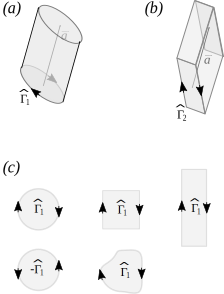
\includegraphics[scale=1.0]{conjugateVectorMeaning}
  \caption{(a) A covariant vector $\op{\Gamma}_1$ can be represented
    by an oriented piece of plane with certain area. Its action on a
    contravariant vector $\vec{a}$ results in a number -- volume of a
    skewed cylinder built by moving the area along the vector. (b) A
    covariant vector $\op{\Gamma}_2$ has different orientation and
    magnitude from $\op{\Gamma}_1$. (c) The shape of the conjugate
    vector (an oriented piece of plane) does not
    matter, as long as its orientation and area stay the same.}
  \label{fig:conjugateVectorMeaning}
\end{figure}
%\begin{tcolorbox}[colback=white!90!ocre, title=Covariant Vectors]
\begin{mybio}{Covariant Vectors}
Contravariant arrow-vectors $\vec{a}$ are oriented line segments
regardless of whether they are in a plane, in three-dimensional space, or in spaces
of higher dimensions.

Covariant vectors\index{Vector!covariant} have different ``structure''
for spaces of different
dimensions. In three dimensions, as we saw, they are oriented
areas. In a plane, they will be oriented line segments similar to
arrow-vectors. In four dimensional space covariant vectors will be
oriented three-dimensional volumes. Thus, unlike contravariant
arrow-vectors, covariant vectors are more difficult to visualize.

The question of geometric meaning of addition of two covariant
vectors -- and other operations on them -- although interesting and
useful, is outside of the scope of this book.
\end{mybio}
%\end{tcolorbox}


\section{Projectors}\label{sec:Projectors}
%% \[
%% \proj{A}\,\projop{A}\,.
%% \]
In many problems it is useful to take a vector $\vec{b}$ and find the
part of it which will be parallel to another vector $\vec{a}$, as illustrated in the
Figure \ref{fig:projector}. This procedure can be described using the
concept of a binary operator. This operator, when given a pair of
vectors $\vec{a}$ and $\vec{b}$, returns the ``component'' of
$\vec{b}$ oriented along $\vec{a}$ -- a \emph{projection}\index{Vector!projection} of $\vec{b}$
onto $\vec{a}$:
\[
\op{P}\, \vec{a}\, \vec{b} = \vec{b}_\parallel\,,
\]
where $\vec{a}$ is parallel to $\vec{b}_\parallel$.

\begin{figure}[htbp]
  \centering
  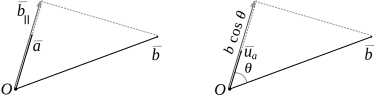
\includegraphics[scale=1.0]{projector}
  \caption{A vector $\vec{b}$ has the ``component'' $\vec{b}_\parallel$ along a given vector
    $\vec{a}$. The length of this components is $b\cos\theta$ where
    $\theta$ is the angle between vectors $\vec{a}$ and $\vec{b}$.}
  \label{fig:projector}
\end{figure}

From the Figure \ref{fig:projector}, it is clear that
\[
\vec{b}_\parallel = \vec{u}_a b\cos\theta = \frac{\vec{a}}{a}\,b\cos\theta\,,
\]
where $\vec{u}_a$ is a unit-length vector parallel to $\vec{a}$.

The right-hand side of the last expression can be written using
dol-operator $\op{\sigma}$, or even better, using the conjugate
vector notation:
\[
\vec{b}_\parallel = \frac{\vec{a}}{a^2}\,ab\cos\theta\, =
\frac{\vec{a}}{a^2}\,(\vecl{a}\vec{b})\,.
\]
For each vector $\vec{a}$ there exists corresponding projection
operator\index{Operator!projector}
that projects all other vectors onto the direction specified by
$\vec{a}$.
\begin{mybio}{Projector Notation}
A projector operator that projects any vector $\vec{b}$ onto the
direction specified by a vector $\vec{a}$ will be denoted as
$\projop{A}$:
\[
\projop{A}\,\vec{b} = \frac{\vec{a}}{a^2}\,(\vecl{a}\vec{b})\,.
\]
Such projector exists for any non-zero vector $\vec{a}$:
\[
\vec{a}\,\longrightarrow\,\projop{A}\,.
\]
In this notation the same -- but capitalized -- letter is used for the
projector as for the vector. In addition, the capitalized letter is doubly
underlined to remind that we project onto the direction parallel to
the specified vector.

Similarly, we will have other projectors
\[
\vec{b}\,\longrightarrow\,\projop{B},\quad\vec{c}\,\longrightarrow\,\projop{C}\,\ldots
\]
\end{mybio}

Projector $\projop{A}$ corresponding to the vector $\vec{a}$ acts on
an arbitrary vector $\vec{b}$ as
\[
\projop{A}\,\vec{b} = \frac{\vec{a}}{a^2}\,(\vecl{a}\vec{b})\,.
\]
In the argument-free notation, this operator takes the following form:
\[
\colorboxed{red}{
\projop{A} = \frac{\vec{a}}{a^2}\,(\vecl{a}) =
\frac{\vec{a}\vecl{a}}{a^2}.
}
\]
\emph{Note} that the order of the vectors $\vec{a}$ and $\vecl{a}$ in the
last expression is very important because it has completely different meaning
from the expression $\vecl{a}\vec{a}$. Indeed, as we agreed,
the expression
\[
\vecl{a}\vec{a} = \vec{a}\cdot\vec{a} = a^2
\]
yields the length squared of the vector $\vec{a}$. In contrast, the expression
\[
\vec{a}\vecl{a}
\]
works as an operator!

We obtained interesting and useful expression for an operator that
accepts a vector $\vec{b}$ and produces another vector as
the result. This expression involves some kind of ``multiplication''
of a vector $\vec{a}$ and its conjugate $\vecl{a}$:
\[
\vec{a}\vecl{a}\,.
\]
It is our first encounter with \emph{tensor
product}\index{Tensor!product}. We will learn
more about this new type of multiplication below.

\subsection{Projector Components}
To find the components of a projector operator\index{Operator!projector!components}
\[
\projop{A} = \frac{\vec{a}\vecl{a}}{a^2}
\]
in a given basis, we apply it to the basis vectors:
\[
\projop{A}\,\vec{e}_i = \frac{\vec{a}}{a^2}\vecl{a}\vec{e}_i = \frac{a_i}{a^2}\vec{a}.
\]
Expanding the vector $\vec{a}$ in the same basis, we arrive at
\[
\projop{A}\,\vec{e}_i = \frac{a_ia_j}{a^2}\vec{e}_j = \proj{A}_{ij}\vec{e}_j\,,
\]
from which follows the expression for the components
\[
\colorboxed{red}{
  \proj{A}_{ij} = \frac{a_ia_j}{a^2}\,.
}
\]
\begin{exercise}\label{exe:determinantOfProjector}
  Using the components of a projector
  \[
  \proj{A}_{ij} = \frac{a_ia_j}{a^2}\,,
  \]
  calculate its determinant.
\end{exercise}

\begin{mybio}{Symmetry of Projectors}
  From the expression for the components of a projector follows that
  \[
  \proj{A}_{ij} = \proj{A}_{ji}\,,
  \]
  which means that to fully specify its components, we need only 3
  numbers (for vectors in a plane we need $\proj{A}_{11}$,
  $\proj{A}_{12}$, and $\proj{A}_{22}$), as opposed to
  4 numbers required to specify a general linear operator.
\end{mybio}

\subsection{Composition of Projectors*}
The idea of composing two functions - discussed in
subsection \ref{subsec:FunctionComposition} on page
\pageref{subsec:FunctionComposition} - can be extended to
linear operators. That is, some types of linear operators can be
composed\index{Composition!of operators}. Indeed, suppose we have a linear operator
\[
\op{L}\,\vec{a} = \vec{b}
\]
and
\[
\op{M}\,\vec{b} = \vec{c}\,.
\]
We can apply the operators $\op{L}$ and $\op{M}$ sequentially:
\[
\op{M}\,(\op{L}\,\vec{a}) = \vec{c}\,.
\]
This way we obtained a new operator $\op{K}$ which we call
\emph{composition of linear operators} $\op{L}$ and $\op{M}$. The same
notation for composition of operators as for the composition of
functions can be used:
\[
\op{K} = \op{M}\,\circ\,\op{L}\,.
\]
Now we can find the components of the operator $\op{K}$. On the one hand,
\[
\op{K}\,\vec{e}_i = K_{ij}\vec{e}_j\,.
\]
On the other,
\[
\op{K}\,\vec{e}_i = \op{M}\,(\op{L}\,\vec{e}_i)=\op{M}\,(L_{iq}\,\vec{e}_q)\,.
\]
Using the linearity of the operator $\op{M}$, we can write
\[
\op{K}\,\vec{e}_i = L_{iq}\,(\op{M}\,\vec{e}_q)= L_{iq}(M_{qj}\,\vec{e}_j)\,.
\]
We arrive at the following expression of the components of $\op{K}$:
\[
K_{ij} = L_{iq}M_{qj}\,,
\]
where the summation over $q$ is implied according to Einstein's
summation rule. Next let us apply this result to projectors.

Suppose we want to project a vector $\vec{c}$ first on the vector
$\vec{a}$, and then project the result onto the vector $\vec{b}$. We
can do it by sequential application of two projectors:
\[
\projop{A} = \frac{\vec{a}\vecl{a}}{a^2}\quad\textrm{ and }\quad \projop{B} =
\frac{\vec{b}\vecl{b}}{b^2}\,
\]
to the vector $\vec{c}$:
\[
\projop{B}\,(\projop{A}\,\vec{c}) = (\projop{B}\circ \projop{A})\,\vec{c}\,.
\]
Composing two linear operators we obtain another linear operator:
\[
\op{L} = \projop{B}\circ \projop{A}\,.
\]
The components of the product operator $\op{L}$ can be
expressed in terms of the components of the factors -- projectors
$\projop{A}$ and $\projop{B}$:
\[
L_{ij} = \proj{A}_{ik}\proj{B}_{kj} = \frac{a_kb_k}{a^2b^2}a_ib_j\,.
\]
The expression $a_kb_k$ is recognized as the scalar product of the
vectors $\vec{a}$ and $\vec{b}$ in orthonormal basis, so the
components $L_{ij}$ are simply given by
\[
L_{ij} = \lambda\, a_ib_j,\quad \lambda = \frac{\vec{a}\cdot\vec{b}}{a^2b^2}\,,
\]
where $\lambda$ is a scalar value -- a number.

\emph{Note} that $\op{L}=\projop{B}\circ \projop{A}$ is no longer a projector in the
sense in which it was defined earlier. There is no vector $\vec{d}$ such that
\[
L_{ij} = \frac{d_i d_j}{d^2}\,.
\]
The following exercise explores this point.
\begin{exercise}\label{exe:projectorIdempotent}
  (a) Show that a projector
  \[
  \projop{A} = \frac{\vec{a}\vecl{a}}{a^2}
  \]
  has the following property:
  \[
  \projop{A}\circ \projop{A} = \projop{A}\,.
  \]
  (b) Does the result of composition $\op{L}=\projop{B}\circ \projop{A}$ have
  this property?
\end{exercise}

\begin{exercise}\label{exe:projectorsCommutativity}
  Consider the composition
  \[
  \op{M} = \projop{A}\circ \projop{B}\,.
  \]
  Find its components and compare them to the components of
  \[
  \op{L}=\projop{B}\circ \projop{A}\,.
  \]
\end{exercise}

\section{Tensor Product}\label{sec:TensorProduct}\index{Tensor!product}
We arrived at an extremely important idea that will allow
``building'' tensors of various kinds from simple ``ingredients,'' such
as vectors. To begin, let us take a closer look at a projector operator:
\[
\projop{A} = \frac{1}{a^2}\vec{a}\vecl{a}\,,\quad
\proj{A}_{ij} = \frac{1}{a^2}a_ia_j\,.
\]
From the first expression, written without the components, it is clear that
the operator $\projop{A}$ involves a contravariant vector $\vec{a}$ and
its covariant conjugate $\vecl{a}$. This distinction is absent in the
second expression for the components of the operator $\proj{A}_{ij}$, making the
expression for components misleading. To fix this, a special notation
for components is introduced. In this notation, the components of
contravariant vectors are written using superscripts:
\[
\vec{a}\quad\longrightarrow\quad a^i\,,
\]
while the components of covariant vectors are written in the
``usual'' way, as subscripts:
\[
\vecl{a}\quad\longrightarrow\quad a_i\,.
\]
With this in mind, the components of the projector $\projop{A}$ are written in
the following way:
\[
\colorboxed{red}{
  \proj{A}^{i\tus}_{\tus j} = \frac{1}{a^2}a^ia_j\,,
}
\]
Now it should be clear that in the last expression vectors of different
kinds are used: one contravariant, and the other covariant.
The little grey circles surve visual purpose only, they help separate
the first contravariant index from the second covariant one.

\begin{mybio}{Clash of Notation}
The use of superscript to denote components of contravariant vectors
leads to the clash of notations. For example, given
\[
a^2\,,
\]
how should we understand it: length squared of a vector, or its second
component?

Surprisingly, this is not a serious problem at all, since the meaning
of the superscript is usually clear from the context in which such
expressions appears.
\end{mybio}
%\end{tcolorbox}

\subsection{Tensor Product 1}
In the expressions
\[
\projop{A} = \frac{1}{a^2}\vec{a}\vecl{a}\,,\quad
\proj{A}^{i\tus}_{\tus j} = \frac{1}{a^2}a^ia_j
\]
the combination of vectors $\vec{a}\vecl{a}$ and their component expression
$a^ia_j$ represent a mathematical object -- operator in this case
-- that is neither a vector, nor a number. Such ``amalgamation'' of
two vectors into a tensor is called \emph{tensor product}. Tensor
product is a simple and versatile way to construct tensors.

Special notation for tensor product of two vectors exists:
\[
\colorboxed{red}{
  \vec{a}\vecl{a} = \vec{a}\otimes\vecl{a}\,.
}
\]
This separate notation may appear redundant, since we understand from
the order of the vectors $\vec{a}$ and $\vecl{a}$ that the expression
on the left is \emph{not a scalar product}. However, using the infix
operator $\otimes$ is convenient because it allows writing other types of
tensor products with ease and consistency.

\subsection{Tensor Product 2}
Using the tensor product notation, we can write
\[
\vecl{a}\otimes\vec{a}\quad \textrm{or, more generally, }\quad \vecl{b}\otimes\vec{a}\,.
\]
These expressions \emph{represent tensors}, and not scalar products
$\vecl{b}\vec{a}=\vec{b}\cdot\vec{a}$.
The components of a tensor $T=\vecl{b}\otimes\vec{a}$ are as follows:
\[
T^{\tus j}_{i \tus} = b_ia^j\,.
\]
The important fact is reflected in the position of indices of the tensor
$T$: it behaves like covariant vector in the first index, and as
contravariant vector in the second index.

\subsection{Tensor Product 3}
With the help of the infix operator $\otimes$ we can write, without
creating ambiguity, a tensor product of two contravariant vectors:
\[
T = \vec{a}\otimes\vec{b}\,,\quad T^{ij} = a^ib^j\,.
\]
The positions of the indices reflect the fact that this kind of tensor
is contravariant in both of them.

A simplified notation is sometimes used:
\[
\vec{a}\otimes\vec{b} = \vec{a}\vec{b}\,,
\]
 but it may lead to confusion, since the expression
$\vec{a}\vec{b}$ is too similar to the scalar product
$\vec{a}\cdot\vec{b}$, especially when using handwriting. We will
avoid this simplified notation.

\subsection{Tensor Product 4}
The last kind of tensor that we can construct from vectors is given
by the tensor product of two covariant vectors:
\[
T = \vecl{a}\otimes\vecl{b}\,, \quad T_{ij} = a_ib_j\,.
\]
Again, one may encounter expressions like $\vecl{a}\vecl{b}$, but we
will prefer to use the infix operator $\otimes$.

%\begin{tcolorbox}[colback=white!90!ocre, title=Problem]
\begin{exercise}\label{exe:transformation4Kinds}
  Write the transformation rules for tensors of all four kinds
  considered above.
\end{exercise}
%\end{tcolorbox}

\section{Tensors Defined}\index{Tensor!definition}
We are in a good position to summarize our understanding of
tensors. Before we do this, let's quickly review the path we took to
reach this position.

Having defined contravariant and covariant vectors, we examined
natural idea of operators -- functions on vectors. We focused on an
important class operators called linear operators.

We studied linear operators that map vectors to other vectors, like
rotation, and, having examined the transformation of operator
components, derived the first type of transformation (see Section
\ref{sec:ComponentTransformation}). This type of
transformation corresponds to the tensor of mixed kind: contravariant
in the first index and covariant in the second index. Later we
encountered many operators of this kind -- projector operators (see
Section \ref{sec:Projectors}.)

Projector operators are unary linear operators and are built on the
bilinear dol-operator $\op{\sigma}$. This binary operator
introduced to us the idea of conjugate space and unary linear
operators mapping vectors into numbers.

From further analysis of projector operators, we arrived at
the idea of tensor product and unlocked a key method of building
tensors of various kinds. Using a pair of vectors, we listed four
different kinds of tensors: covariant-covariant,
covariant-contravariant, contravariant-covariant, and
contravariant-contravariant. All these tensors can be viewed as
operators acting on vectors, either covariant or contravariant,
depending on the tensor type.

Having reviewed our steps, we can define tensors as follows:
%\begin{tcolorbox}[colback=white!85!ocre, title=Tensor Defintion]
\begin{mydef}{Tensors}
  Tensors are \emph{mathematical objects} with the following essential properties:
  \begin{itemize}
    \item\phantom{x}
\item Tensors can be combined (added) pairwise to yield another tensor.
\item Tensors can be multiplied by real numbers to yield another tensor.
\item Tensors can be represented via components, written relative to some basis.
\item When basis changes, components of tensors transform in a very specific way, to
ensure that the \emph{tensor remains the same}.
  \end{itemize}
  \vspace{0.2cm}
\end{mydef}
%\end{tcolorbox}
This definition is deliberately analogous to the definition of
vectors. In some sense tensors are \emph{next tier vectors}. Tensors
are mathematical objects following vectors in the ladder of
abstraction and power, like vectors are mathematical objects following
numbers in the ladder of abstraction and power.
\subsection{Other Definitions}
Let us revisit the definitions of tensors given in the
introduction. The first one read:
%\begin{tcolorbox}[colback=white!85!ocre, title=Tensors Definition 1]
\begin{mydef}{Tensors Definition 1}
Tensor on a vector space $V$ over a field $k$ is an element $t$ of the vector space
\begin{equation*}
	T^{p,q} (V) = (\otimes^p V)\otimes (\otimes^q V^*)\,,
\end{equation*}
where $V^*=\textrm{Hom}(V, k)$ is the dual space of $V$.
\vspace{0.2cm}
\end{mydef}
%\end{tcolorbox}
In this definition the set of vectors $V$, which we denoted as $\vsp{A}$,
is called \emph{vector space}. Recall that vectors and operation with
vectors require numbers. Numbers, which can be added, multiplied in a
usual way, form what mathematicians call \emph{field}\index{Field}. Therefore,
all vectors taken together are technically called
``vector space $V$ over a field $k$.''

Next, the use of the operator of tensor product $\otimes$ in the
definition makes more sense, since it is the basic way to build
tensors from vectors. Notice that two types of vectors are mentioned:
one from the vector space $V$, and the other from its conjugate (dual)
-- vector space $V^*$; in our notation $V^*=\vspd{A}$. The conjugate
vectors behave very much like vectors from the original vector space:
they can be added, multiplied by numbers, expanded in their own basis,
and so on. This close correspondence between vector space and its conjugate
is called \emph{homomorphism}\index{Homomorphism}\footnote{From Greek
\emph{homos} (same) and \emph{morphe} (shape).} and denoted
$\textrm{Hom}(V, k)$.

Tensor of the kind $T^{p,q}(V)=(\otimes^p V)\otimes (\otimes^q V^*)$ has $p$
contravariant indices and $q$ covariant indices. We mostly dealt with
tensors with the following types: $T^{1,1},\,T^{0, 2}\,, T^{2, 0}$.

Finally, tensors are vectors because they can be added, multiplied by
numbers, have components, and have vector-like transformation
rules. Tensors of a given type, e.g. $T^{2, 1}$, taken together, form
a vector space; there is a separate vector space for each type of
tensor.
\begin{center}
\line(1,0){4in}
\end{center}
\vspace{0.5cm}
The second defintion stated:
%\begin{tcolorbox}[colback=white!85!ocre, title=Tensors Definition 2]
\begin{mydef}{Tensors Definition 2}
An $n$th-rank tensor in $m$-dimensional space is a mathematical object
that has $n$ indices and $m^n$ components and obeys certain
transformation rules.
\vspace{0.2cm}
\end{mydef}
%\end{tcolorbox}
Here tensor is mentioned in connection with some $m$-dimensional
space, which we recognize as the underlying vector space
$\vsp{A}$\index{Vector!space}. In
our case the number of dimensions, given by the number of independent
directions, equals 2.

The rank of a tensor\index{Tensor!rank} is given by the number of indices, or the number
of vectors that go into the tensor product. For example:
\[
L=\vecl{a}\otimes\vecl{b}\,\longrightarrow\, L_{ij}\quad \textrm{ is
  the tensor of the second rank,}
\]
\[
M=\vecl{a}\otimes\vecl{b}\otimes\vec{c}\,\longrightarrow\,
M_{i\,\,j\,\tus}^{\tus\tus k}\quad \textrm{ is the tensor of the third rank.}
\]
Since the value of each index runs from 1 to $m$, where $m$ is the
dimension of the vector space, tensors of the rank $n$ should have
$m^n$ components in total. The essential property of tensor components
is how they are transformed when the basis changes -- the tensor
transformation rule.
\begin{center}
\line(1,0){4in}
\end{center}
\vspace{0.5cm}
The last definition, given in the introduction, looks as follows:
%\begin{tcolorbox}[colback=white!85!ocre, title=Tensors Definition 3]
\begin{mydef}{Tensors Definition 3}
Just as a \emph{vector} is a mathematical quantity
that describes translations in two- or three-dimensional
space, a tensor is a mathematical quantity used to
describe general transformations in $n$-dimensional
space. Precisely, if the locations of points in $n$-dimensional
space are given in one coordinate system by
$(x^1,x^2,…,x^n)$ and in a transformed coordinate system
by $(y^1, y^2,…,y^n)$ (it is convenient to use superscripts
rather than subscripts), then a “rank 1 contravariant
tensor” is a quantity $T$, with single components, that
transforms according to the rule:
\begin{equation*}
	T^i_{new} = \sum\limits_{r=1}^{n} \frac{\partial y^i}{\partial x^r} T^r\,.
\end{equation*}
\vspace{0.2cm}
\end{mydef}
%\end{tcolorbox}

We now know that tensors can be used to describe transformation of one
vector into another (e.g. projectors). Similar ideas can be applied
to vectors in spaces with higher dimensions. In this sense, tensors
can describe general transformaions in $n$-dimensional space.

The essential property of tensor components is their tranformation
rule. In this definition a transformation rule for a tensor of the
first rank (a usual vector) is given:
\[
T^{'i} = Z^i_{\phantom{x}r}T^r\,,
\]
where the set of numbers $Z^i_{\phantom{x}r}$ describes the relation
between the ``old'' basis (coordinates $x$) and the ``new'' basis
(coordinates $y$).

\section*{Chapter Highlights}
{\setstretch{1.5}\chhc
  \it
  \small
\begin{itemize}
\item Two vectors can be compared for similarity by calculating the
  ``degree of overlap''. The longer two vectors are and the closer
  their mutual direction -- the greater the overlap is.
\item Degree of overlap can be described by a binary linear operator
  $\op{\sigma}$. This operator is closely related to the concept of
  scalar product of two vectors.
\item When scalar product (or, equivalently, degree of overlap) is
  defined for vectors, each vector receives a ``special relative'' --
  conjugate vector -- that lives in different vector space, called
  conjugate or dual space.
\item When the degree-of-overlap operator $\op{\sigma}$ is partially
  applied, the result is a unary linear operator that yields a number
  for every input vector. Importantly, such an operator is also a
  vector, albeit not an arrow-like vector.
\item Unary linear operators that act on arrow-like vectors themselves
  form a space of vectors. The latter vectors are conjugate to the
  ``usual'' space of  arrow-like vectors.
\item If arrow-like vectors are contravariant vectors, then their
  conjugate counterparts are covariant vectors. Covariant vectors can
  be represented geometrically as oriented area elements (for three
  dimensional space).
\item Projectors are unary linear operators that act on input arrows
  to yield another arrow that is parallel to a certain
  direction. Projectors are degenerate operators.
\item Projectors can be written using the efficient tensor product
  notation.
\item Tensor product is a simple and powerful way to build up tensors
  of any rank and kind from a number of covariant and contravariant
  vectors.
\item Tensors are mathematical objects with many properties similar to
  vectors. However, their rank is higher and tensors can be used to
  express linear relations between vectors.
\end{itemize}

}
